
\chapter{Running the Grover Search Algorithm} \label{chapter:grover_algorithm}

This chapter describes an experimental implementation of the so-called {\it Grover search algorithm} with our two-qubit quantum processor. The first section provides a short introduction of the algorithm and motivates the interest in realizing it. The following sections then discuss the details of its experimental realization. We show the results that we obtained and compare the algorithm fidelity and efficiency to that of an equivalent, classical algorithm. Finally, we analyze all relevant unitary and non-unitary error sources relevant to our experiment and provide a quantitative error model of our implementation of the algorithm.

\section{Introduction \& Motivation}

Search algorithms are of great importance in many domains of mathematics and computer science. One such search problem that often arises and which will be discussed in the following sections can be formulated in simple terms as follows:

\smallskip

Assume that we have a search space $\begin{mathcal}S\end{mathcal}$ that consists of a finite number $N$ of states $s \in \begin{mathcal}S\end{mathcal}$. The solution to our search problem corresponds to a subset of $M$ states of the search space $\begin{mathcal}T\end{mathcal} \subset \begin{mathcal}S\end{mathcal}$. We can then define a search function $\Or(s):\begin{mathcal}S\end{mathcal}\to \{0,1\}$ that discriminates between states that solve the search problem and states that don't, such that $\Or(s) = 1$ for $s \in \begin{mathcal}T\end{mathcal}$ and $\Or(s) = 0$ otherwise. In accordance with the general convention in the literature on the Grover search algorithm, we will  often refer to this search function as the {\it Oracle function} or (in a quantum-mechanical context) as the {\it Oracle operator}.

\smallskip

Using this definition of the search problem, the goal of a search algorithm is to find all states $t\in\begin{mathcal}S\end{mathcal}$ for which $\Or(t) = 1$. In the following, for the sake of simplicity we assume that the solution set $\begin{mathcal}T\end{mathcal}$ contains only one single state $t$. This special case can be generalized to cases where more than one solution to the search problem exists (see e.g. \cite{nielsen_quantum_2000,mermin_quantum_2007} for a detailed review)

\smallskip

The first step in order to solve a search problem of the kind described above using classical or quantum computation is to map the problem to a form suitable for solution by a digital (quantum) computer. For this, we first number and encode the $N$ input states $i \in \begin{mathcal}S\end{mathcal}$ in binary form as $i=(b^i_l,\hdots,b^i_0)_B$, where $l$ is the length of the binary register able to hold all $N$ input states. With this definition, it is then trivial to find a mathematical representation of $\Or$ that operates on a binary input register. 

\smallskip

Using these assumptions and definitions, it can be shown that the most efficient classical search algorithm for solving the search problem above will use $\begin{mathcal}O\end{mathcal}(N)$ calls of the function $\Or$ to find the solution of the search problem. If assuming that calling $\Or$ is much more ``expensive'' in time or resources than any other operation, $\begin{mathcal}O\end{mathcal}(N)$ will then also correspond to the overall computational efficiency of the algorithm.

\smallskip

Amazingly, in 1997, Lov Grover found a quantum algorithm that could solve this search problem with only $\begin{mathcal}O\end{mathcal}(\sqrt{N})$ calls to the function $\Or$ \citep{Grover_Quantum_1997}. His algorithm achieves this by repeatedly calling a quantum-mechanical implementation of the function $\Or$, starting from a highly superposed qubit register $\sum\limits_i^N \ket{i}$ and applying a special operator to the resulting output state afterwards. The individual steps of his algorithm are given as follows:

\begin{enumerate}
 \item Initialize a qubit register to the state $\ket{\psi} = \ket{0}$ (corresponding to a binary input state $\ket{0000\hdots0_B}$)
 \item Apply the generalized Hadamard operation to the qubit register, producing a fully superposed quantum state $$\ket{\psi} = \frac{1}{\sqrt{N}}\sum\limits_{i=0}^{N-1} \ket{i}$$
 \item Repeat the following sequence $\begin{mathcal}O\end{mathcal}(\sqrt{N})$ times:
 \subitem a) Apply the {\it Oracle operator} $\ket{i}\to (-1)^{\Or(i)}\ket{i}$.
 \subitem b) Apply the so-called {\it diffusion operator} $\ket{i} \to -\ket{i}+\frac{2}{N}\sum\limits_{j=0}^{N-1}\ket{j}$.
	\item Measure the state of the quantum register in the computational basis $\ket{i}$.
\end{enumerate}

Note that for the description above we have enumerated the states of the qubit register from $\ket{0}$ to $\ket{N-1}$. The Grover algorithm makes use of quantum parallelism to solve the search problem $\begin{mathcal}O\end{mathcal}(\sqrt{N})$ times faster than the most efficient classical algorithm. To understand better the strategy it uses, the different steps of the algorithm can be rephrased in the following, more general way:

\begin{itemize}
\item First, the algorithm creates a fully superposed quantum state which contains all possible solutions to the search problem at once. The amplitudes and phases of each individual state are all equal in the beginning.
\item Then, it applies the Oracle operator to this superposed state. The effect of the Oracle is to turn the phase of the state $t$ for which $\Or(t)=1$ by an angle $\pi$. As will be shown later, such an Oracle operator can be implemented in a straightforward way for any classical search function.
\item In the next step, it applies a diffusion operator to the quantum state which transfers a fraction of the amplitude from states with zero phase to the states with $\pi$ phase, increasing thus the amplitude of the latter. In this process, the phases of all states get also turned back to zero, allowing the algorithm to repeat the sequence above.
\item Repeating these two operations increases each time the amplitude of the states that correspond to a solution of the search problem until the amplitudes of all the other states vanish. After that point, the process reverses and the amplitude is transferred back to the original states. It is therefore crucial to stop the repetition sequence given above after the right number of iterations.
\end{itemize}

By implementing the search function as a quantum operator acting on a superposition, the Grover algorithm is able to somehow evaluate it in one single call for all possible input states. This so-called {\it quantum parallelism} provides the basis for the speed-up of the search in comparison to a classical algorithm. However, being able to encode the result of the search function in the phase of a multi-qubit state does not directly translate to a speed advantage since it is usually very hard to extract this phase information from the quantum state. Indeed, to extract the values of all phases from an $N$-qubit state, it would be necessary to perform $\begin{mathcal}O(2^N)\end{mathcal}$ measurements on an ensemble of such identically prepared quantum states. However, extracting the amplitudes from such a state takes only $\begin{mathcal}O\end{mathcal}(N)$ measurements, that in addition can usually be carried out in parallel. It is for this reason that the Grover algorithm uses an operator that transforms the information encoded in the phases of the qubits to an information encoded in their amplitude. However, since the conversion between phase to amplitude information through the application of an unitary operator is limited by certain physical constraints, the algorithm needs to repeat the encode-and-transfer sequence described above $\begin{mathcal}O(\sqrt{N})\end{mathcal}$ times. \cite{lloyd_quantum_1999,meyer_sophisticated_2000,lanyon_experimental_2008,ahn_information_2000,ding_review_2007,linden_good_2001,braunstein_speed-up_2002}

\smallskip

To analyze further the constraints and principles of the algorithm, we will discuss a more detailed derivation of it starting from the Schrödinger equation and we will also explain what limits the efficiency of the phase-to-amplitude conversion in the algorithm.

\subsection{Deriving the Grover Algorithm from Schrödinger's Equation}


An interesting derivation of the Grover algorithm starting from Schrödinger's equation has been detailed by Grover himself in a seminal paper \citep{grover_schrodingers_2001} and shall be briefly rediscussed here since it sheds light on the basic principles on which the algorithm is based. The derivation begins by considering a quantum system governed by Schrödinger's equation, which can be written as (setting $\hbar = 1$ for better readability)
%
\begin{equation}
-i\frac{\partial}{\partial t}\psi(x,t) = \frac{\partial^2}{\partial x^2}\psi(x,t)-V(x)\psi(x,t) \label{eq:grover_derivation}
\end{equation}
%

\begin{wrapfigure}{r}{6cm}
\vspace{-1cm}
\includegraphics[width=5.2cm]{"./material/papers/grover/grover_derivation_schroedinger"}
\caption{Wave function $\psi(x)$ and potential $V(x)$ defined on a grid of points $x_1,\hdots,x_N$. A minimum of the potential can encode a search value $x_i$.}
\label{fig:GroverDerivationSchroedinger}
\end{wrapfigure}


Here $\psi(x,t)$ describes the wave-function and $V$ is a time-independent potential. Let us assume that the potential $V(x)$ is shaped as in fig. \ref{fig:GroverDerivationSchroedinger}, i.e. possessing a global minimum of energy. When one initializes the system to a state $\psi_0(x,t_0)$ and lets it evolve for a given time, $\psi(x,t)$ will be attracted by the minimum of potential energy and ``fall into it'' much like a classical particle in such a potential would\footnote{Of course, since there is no dissipation, the state will not come to rest at the minimum point of energy but rather oscillate around it conserving its total potential and kinetic energy.}. We might thus ask if we can encode the solution to a search problem as a point of minimum energy $x_0$ of a potential $V(x)$, take an initial state $\psi_0(x,t_0)$ and let it evolve into a state that has a high probability around $x_0$, thereby solving the search problem. To answer this question, it is first necessary to discretize the wave function $\psi(x,t)$ such that it can represent the search problem stated in the last section, and which is defined over a finite number of states. In the most simple case, we can use a regular grid of points $x_i$ with a spacing $\Delta x$ for this, as shown in fig. \ref{fig:GroverDerivationSchroedinger}b. Discretizing the time evolution of eq. \ref{eq:grover_derivation} in steps $\Delta t$ as well and defining $\epsilon = \Delta t/\Delta x^2$, we obtain a new equation of the form
%
\begin{equation}
-\frac{\psi_i^{t+\Delta t}-\psi_x^{t}}{\Delta t} = \frac{\psi_{i+1}^t+\psi_{i-1}^t-2\psi_x^t}{\Delta x^2} -V(x_i)\psi_i^t
\end{equation}
%
where we have written $\psi(x_i,t)=\psi_i^t$. For a circular grid with $N$ points we can write this equation in matrix form as
%
\begin{equation}
\vec{\psi}^{t+\Delta t} = S^{\Delta t}  \cdot \vec{\psi}^t
\end{equation}
%
with $S$ being a state transition matrix of the form
%
\begin{equation}
S^{\Delta t} = \left(
	\begin{array}{ccccc}
		1-2i\epsilon-iV(x_1)\Delta t & i\epsilon & 0 & \hdots &  i\epsilon \\
		i \epsilon & 1-2i\epsilon -iV(x_2)\Delta t & i\epsilon & \hdots & 0 \\
		0 & i\epsilon & \ddots & & \vdots \\
		\vdots & & & \ddots  & \vdots \\
		i \epsilon & 0 & \hdots & i\epsilon & 1 - 2i\epsilon -iV(x_N)\Delta t
	\end{array}
 \right) \label{eq:grover_iteration_matrix}
\end{equation}
%
For infinitesimal times $\Delta t$ we can separate the effect of the potential $V(x)$ on the wave function from the spatial dispersion $\propto i\epsilon$ by writing $S^{\Delta t} \approx D\cdot R$ with 
%
\begin{eqnarray}
D & = & \left( 
		\begin{array}{cccccc}
		1-2i \epsilon & i\epsilon & 0 & 0 & \hdots & i\epsilon \\
		i \epsilon & 1 - 2i \epsilon & i \epsilon & 0 & \hdots & 0 \\
		\hdots & \ddots & & & & \vdots \\
		i \epsilon & 0 & 0 &  \hdots & i\epsilon & 1-2i \epsilon \\
		\end{array}
	\right)
\end{eqnarray}
%
and 
%
\begin{eqnarray}
R & = & \left( \begin{array}{ccccc}
	e^{-i V(x_1) \Delta t} & 0 & \hdots & 0 \\
	0 & e^{-i V (x_2) \Delta t} & \hdots & 0 \\
	0 & \hdots & & 0 & e^{-i V (x_N) \Delta t} \\
	\end{array}
	\right)
\end{eqnarray}
%
This approximation is correct to order $\begin{mathcal}O\end{mathcal}(\epsilon)$ up to an irrelevant renormalization factor. Now, we can repeatedly apply the matrix product $D\cdot R$ to the wave function to obtain its state after a given finite time $t$ by writing
%
\begin{equation}
\vec{\psi}^{t_0+t} = \left(\prod\limits_{i = 1}^{t/\Delta t} D\cdot R\right)\cdot \vec{\psi}^{t} \label{eq:trotter_evolution}
\end{equation}
%
This technique of splitting up the full evolution operator into a product of two or more non-commuting operators that are applied repeatedly to the wave function to obtain its state after a finite time is sometimes referred to as {\it Trotterization} -- in reference to the so-called {\it Lie-Trotter formula} on which it is based -- and on which digital quantum simulation relies\citep{lloyd_universal_1996,lanyon_universal_2011}.

\smallskip

As can be seen in eq. (\ref{eq:trotter_evolution}), the evolution of the wave function at infinitesimal times is governed by two processes: The interaction with the potential $V$ and a diffusion process that mixes different spatial parts of the wave function with each other. The operator $D$ resembles a Markov diffusion process since each row and column of the matrix sums up to unity, whereas $R$ changes the phase of each element of the wave function as a function of the local potential seen by it. If we apply $R$ to a fully superposed initial state of the form $\psi_i = 1$ (omitting the normalization factor for simplicity) and assume that $V_i = 0$ for $i \ne j$ and $V_j \Delta t = \pi/2$ (the potential thus encoding a search function with $\Or(j)=1$ and $\Or(i)=0$ for $i\ne j$), the element $\psi_j$ will get turned according to $\psi_j \to i\psi_j $, whereas all other elements $\psi_i$ will remain unchanged. Applying the operator $D$ to the resulting state will transform $\psi_j$ according to $\psi_j \to \psi_j(i+2\epsilon(1+i))$ with a corresponding amplitude $\sqrt{1+4\epsilon+\begin{mathcal}O\end{mathcal}(\epsilon^2)}$ and the adjacent states $\psi_{j\pm 1}$ according to $\psi_{j\pm 1} \to \psi_{j\pm 1}(1-\epsilon(1+i))$ with an amplitude $\sqrt{1-2\epsilon +\begin{mathcal}O\end{mathcal}(\epsilon^2)}$. Hence there is a transfer of amplitude between the state whose phase has been turned and its neighboring states. If we reset the phases of all the $\psi_i$ to zero afterwards, we can iterate the application of $D\cdot R$ until all of the amplitude has been transferred to the element $\psi_j$ which corresponds to a solution to the search problem. This is, in essence, exactly what the Grover algorithm does, the only difference being that it replaces the matrix $D$ with an unitary matrix that maximizes the amplitude transfer to the states solving the search problem, thereby speeding up the algorithm. As stated before, the efficiency with which the algorithm can transfer amplitude between different states is limited by physical constraints. In the next section, we will therefore discuss exactly what limits this efficiency and which unitary diffusion matrix one should choose to maximize it.

\subsubsection{Efficiency of Quantum Searching}

As discussed by L. Grover \citep{grover_schrodingers_2001}, it is interesting to ask what is the maximum amount of amplitude that can be transferred in a single step of the Grover search algorithm and which matrix $D$ should be chosen to maximize this transfer. To answer this question and derive the ideal diffusion matrix, we will assume first that, without loss of generality, the matrix $R$ which encodes the value of the search function $\Or$ in the quantum state of the qubit register can be written as
%
\begin{eqnarray}
R & = & \begin{mathrm}I\end{mathrm}-2\sum\limits_{j=0}^{N-1} \Or(j)\ket{j}\bra{j}. \label{eq:GroverOracleFunction}
\end{eqnarray}
%
This operator will flip the sign of all states for which $\Or(j) = 1$. Now, the next step consists in finding a diffusion or state transfer matrix which will maximize the amplitude transfer to states tagged by the Oracle operator above and which will also reset the phases of the quantum register to zero afterwards, such that we might apply the Oracle operator to the resulting state again. In the most general case, such a state transfer matrix will have the form
%
\begin{equation}
D_c = \left(	
	\begin{array}{ccccc}
		b & a & a & \hdots & a \\
		a & b & a & \hdots & a \\
		\vdots & & \ddots &  &\vdots \\
		a & & \hdots & a & b \\
	\end{array}
\right).
\end{equation}
%
Here, we assume that all non-diagonal elements of the matrix are equal, which is well justified since we have no knowledge of the structure of the search space of the problem and therefore want to treat all basis states equally during the phase-to-amplitude conversion. Furthermore, since both the initial quantum state and the Oracle operator as given by eq. (\ref{eq:GroverOracleFunction}) contain only real numbers and we demand that the quantum state after applying $D_c$ may contain only positive real numbers as well it is easy to show that $a,b$ must be real numbers. Finally, the unitarity of quantum operators demands that $D_c^\dagger D_c = \begin{mathrm}I\end{mathrm}$, which for the matrix above is equivalent to the two conditions
%
\begin{eqnarray}
 1 & = & b^2+(N-1)a^2, \\
0 & = & 2ab +(N-2)a^2.
\end{eqnarray}
%
Solving these two equations for $a,b$ yields the trivial solution $b = \pm 1$, $a = 0$ and the more interesting one $b = \pm(1-2/N)$, $a=\mp 2/N$. As can be checked easily, the solution $b = 1-2/N$, $a = 2/N$ results in a maximum amplitude transfer from states $\ket{i}$ for which $\Or(i)=0$ to states $\ket{j}$ for which $\Or(j)=1$. Thus the ideal diffusion matrix to be used in the Grover algorithm is given as
%
\begin{equation}
D = \left( \begin{array}{ccccc}
	-1+2/N & 2/N & 2/N & \hdots & 2/N \\
	2/N & -1 + 2/N & 2/N & \hdots & 2/N \\
	\vdots & & \ddots &  & \vdots \\
	2/N & 2/N & 2/N & \hdots & -1 + 2/N \\ 
	\end{array} \right). \label{eq:GroverDiffusionOperator}
\end{equation}
%
This matrix, together with an Oracle operator $R$ as given by eq. (\ref{eq:GroverOracleFunction}) will yield the maximum amplitude transfer from states not solving the search problem to states that solve it. Repeating the application of $D\cdot R$ on an initially fully superposed quantum state for $\begin{mathcal}O\end{mathcal}(\sqrt{N})$ times will transform the input state to a state containing only the solutions of the search problem.

\smallskip

For the two-qubit case, the Oracle and diffusion operators $R$ and $D$ of the previous sections are
%
\begin{eqnarray}
	R  & = & \left( \begin{array}{rrrr} (-1)^{\Or(00)} & 0 & 0 & 0 \\ 0 & (-1)^{\Or(01)} & 0 & 0 \\ 0 & 0 & (-1)^{\Or(10)} & 0 \\ 0 & 0 & 0 & (-1)^{\Or(11)} \end{array} \right), \label{eq:two_qubit_oracle_operator} \\
  D  & = & \frac{1}{2}\left( \begin{array}{rrrr} -1 & 1 & 1 & 1 \\ 1 & -1 & 1 & 1 \\ 1 & 1 & -1 & 1 \\ 1 & 1 & 1 & -1 \end{array} \right). \label{eq:two_qubit_diffusion_operator} 
\end{eqnarray}
%
Before discussing the experimental implementation of this algorithm, we will show how we can compare its computational efficiency to that of an equivalent classical algorithm in order to assess the achieved quantum speed-up.

\subsection{Comparison to Classical Algorithms}

To be able to compare the Grover algorithm as outlined here to a classical version solving the same search problem, we will now discuss another variant of the algorithm that uses an ancilla qubit to encode the result of the search function. This implementation will make it possible to devise a classical algorithm that can be directly compared to the quantum algorithm. 

\subsection{Ancilla-based Implementation of the Algorithm}

\begin{figure}[ht!]
	\centering
		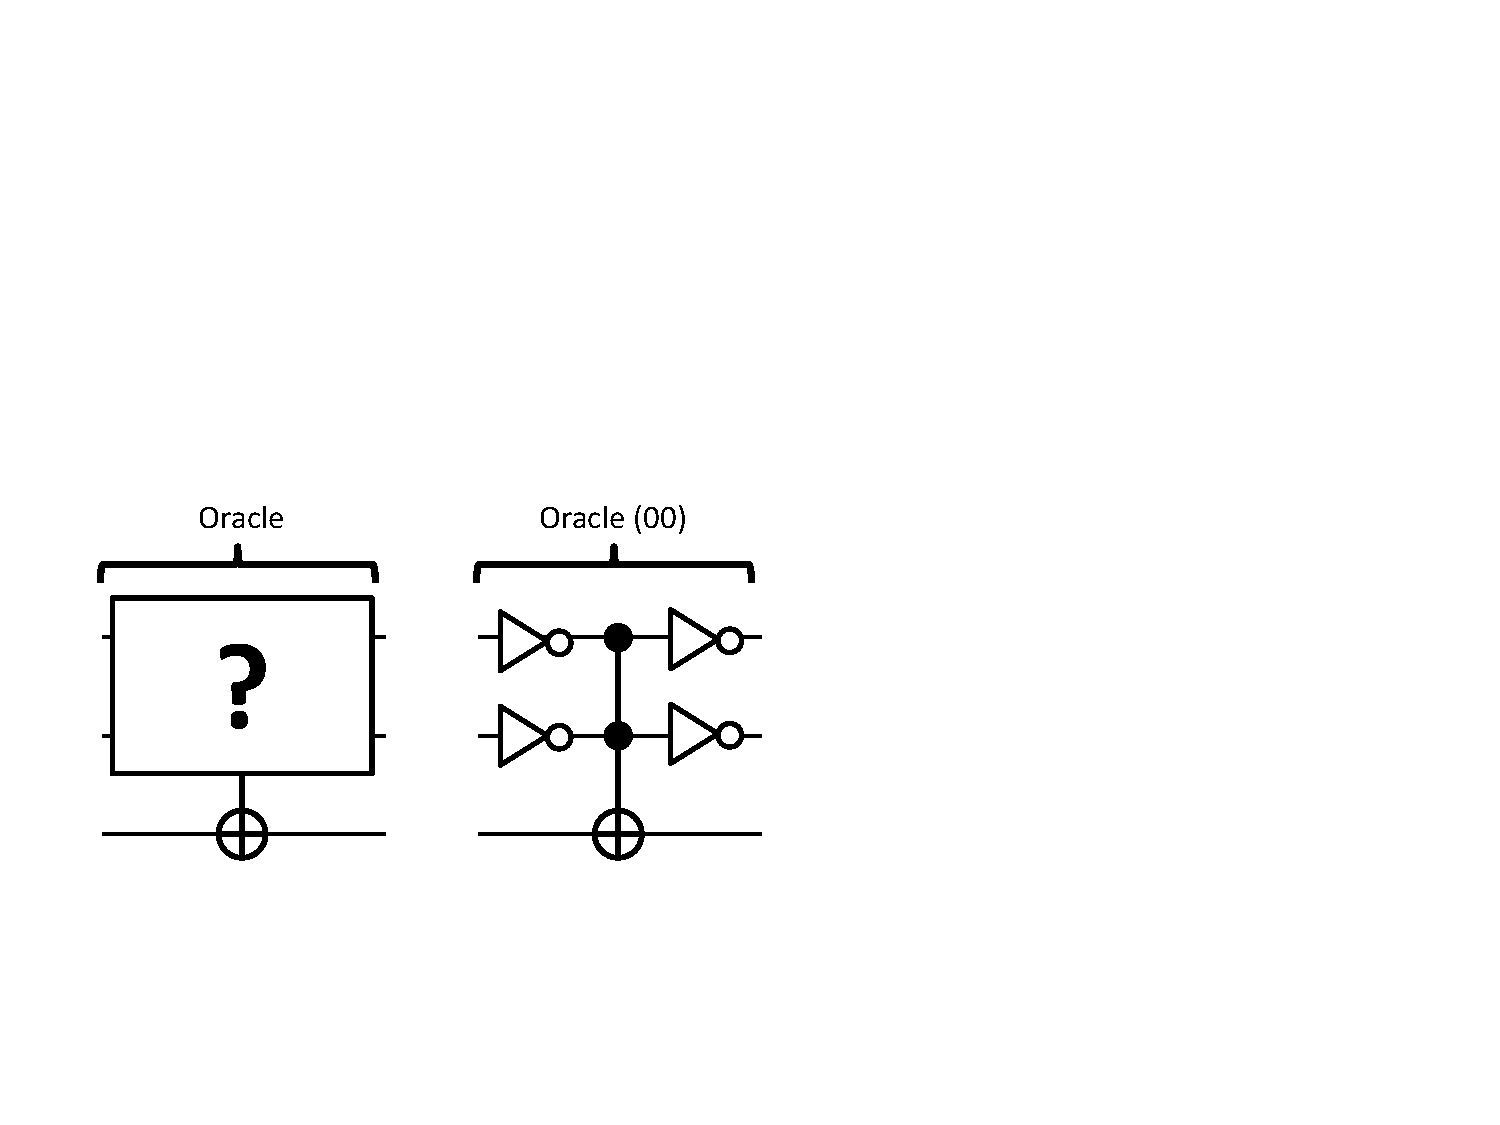
\includegraphics[width=0.8\textwidth]{./material/papers/grover/different_oracle_implementations}
	\caption[]{a) Definition of the NOT logic gate used in the following diagrams. b) Ancilla-based implementations of the Oracle functions $\Or$ for two qubits. The state of the third bit get flipped if the search function $\Or(i)=1$ for the given input state $i$. c) Example of an ancilla-based search function returning a true value for the input state $00$.}
	\label{fig:GroverOracleImplementations}
\end{figure}

The implementation of the Grover search algorithm as outlined above encodes the value of the search function $\Or$ directly in the phase of the input state supplied to this function. This makes it hard to compare the algorithm to a classical search algorithm which operates on a binary input state and, in general, cannot encode the result of the search function directly in this state. It is therefore useful to formulate a version of the Grover algorithm where the Oracle function does not directly encode the tagged state in the input qubit register but rather uses an ancilla qubit to store the result of calling $\Or$. Such a representation of the algorithm, although of little practical relevance, is useful since it allows us to directly compare the quantum algorithm to a classical counterpart implemented using reversible logic gates, thus making it possible to benchmark the quantum algorithm and provide an estimation of the quantum speed-up that can be achieved.

\smallskip

Exemplary implementations of ancilla-based search functions $\Or$ implemented using reversible (quantum) gates are shown in fig. \ref{fig:GroverOracleImplementations} for the two-qubit case. There, a three-qubit Tofolli gate in combination with several single-qubit NOT gates (that can be easily implemented as single-qubit $X_{\pi}$ rotations) are used to flip the state of an ancilla-qubit conditionally on the input state of the gate. Using a similar approach, any arbitrary classical search function $\Or$ that can be implemented with a set of universal reversible logic gates (e.g. the Toffoli gate and the NOT gate) can be directly mapped to a corresponding quantum operator that works on quantum-mechanical input states and implements the classical search function.

\begin{figure}[ht!]
	\centering
		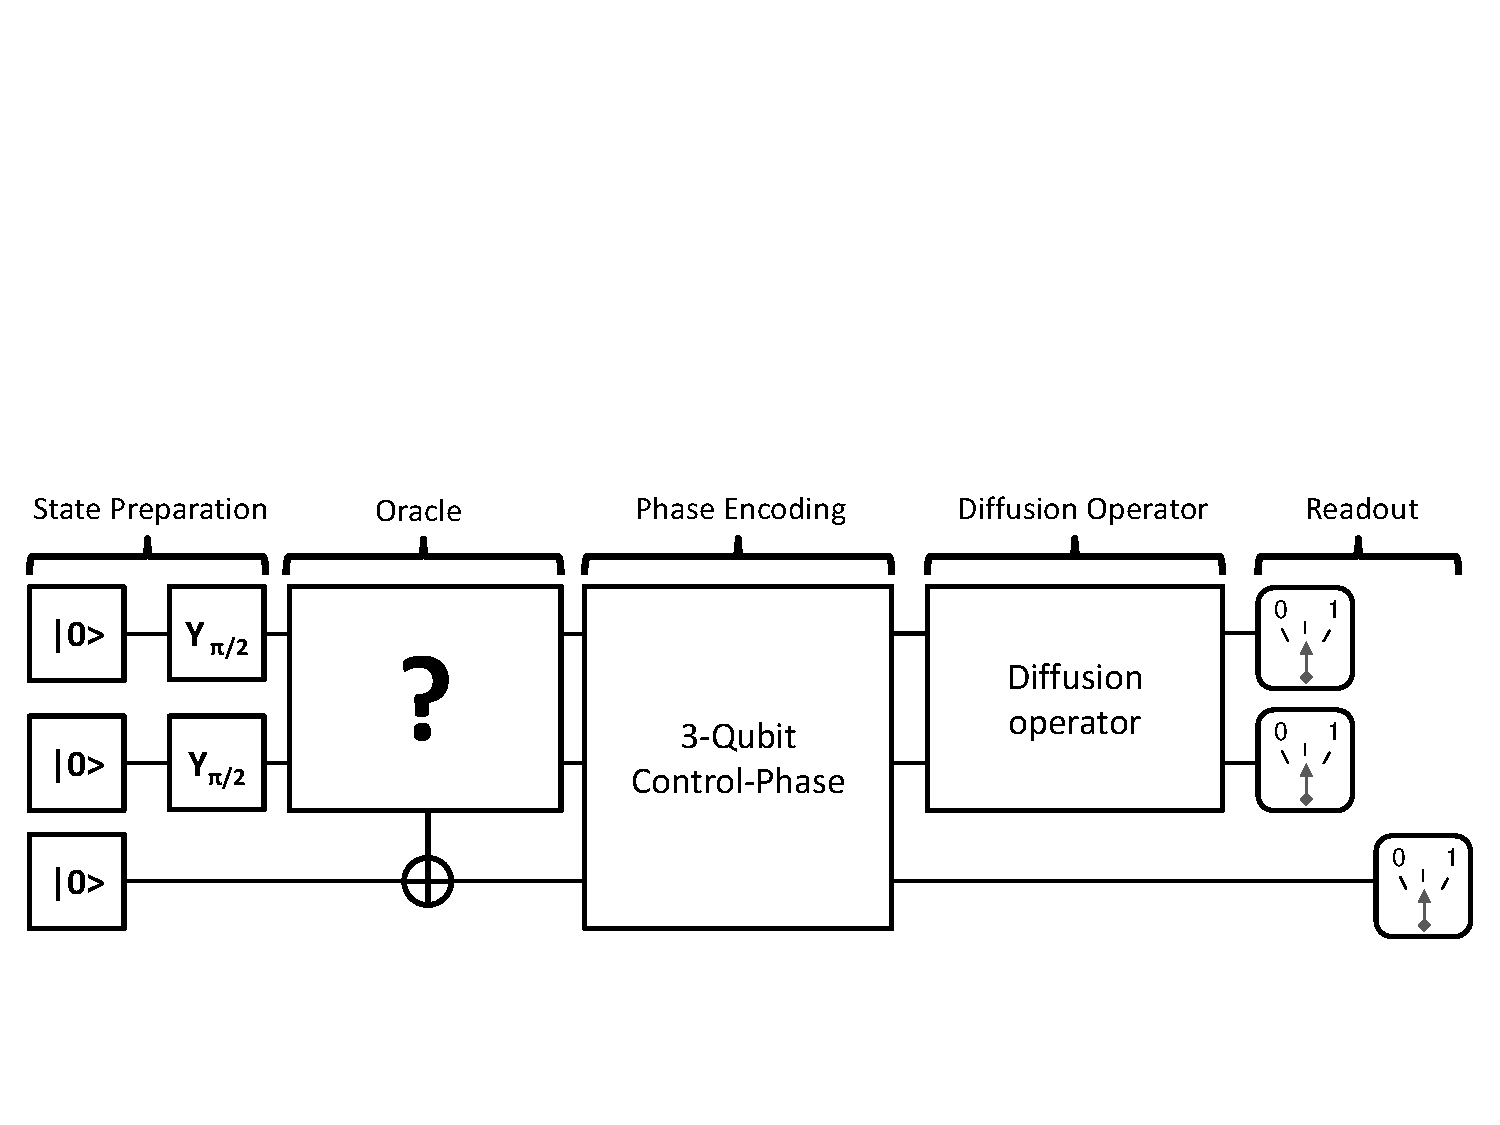
\includegraphics[width=1\textwidth]{./material/papers/grover/quantum_algorithm_full}
	\caption{Full version of an ancilla-based implementation of the two-qubit Grover search algorithm. The algorithm flips the state of a (third) control qubit for one of the four possible input states in accordance to an unknown Oracle function. It then applies a three-qubit control-phase operation of that maps $\ket{xy1}\to -\ket{xy1}$, $\ket{xy0}\to\ket{xy0}$ to encode the state of the control qubit directly in the two input qubits. Then, a diffusion operator is used to determine the state which has been tagged by the Oracle function.}
	\label{fig:GroverAlgorithmFullSchematic}
\end{figure}

\smallskip

Now, to use the Grover algorithm with such an ancilla-based quantum Oracle, it is necessary to re-encode the result of the Oracle in the qubit input state. Figure \ref{fig:GroverAlgorithmFullSchematic} shows a version of the two-qubit Grover algorithm that achieves exactly this by using a three-qubit control-control-not (CCNOT) gate $C$ of the form
%
\begin{equation}
C = \mathrm{I}^{8\otimes 8}-2\sum\limits_{ij} \ket{ij1}\bra{ij1}.
\end{equation}
%
After the re-encoding of the result, the ancilla qubit is not needed during the remainder of the algorithm but must not be read out before the algorithm terminates. A discussion of possible realizations of the ancilla-based Oracle operator can also be found in \citep{mermin_quantum_2007}.

\subsection{Comparison to a Classical Algorithm}

\begin{figure}[ht!]
	\centering
		\includegraphics[width=1.0\textwidth]{"./material/papers/grover/classical_reversible_algorithm"}
	\caption{Classical reversible implementation of a query-and-guess search algorithm on a two-bit input register. An exemplary Oracle function can be implemented using two single-bit NOT operations and a Toffoli gate. R designates the generation of a random binary value at the beginning of the algorithm. If the Oracle does not yield the correct answer, the test state is incremented. The average success probability of the algorithm is 50 \%.}
	\label{fig:GroverClassicalReversibleAlgorithm}
\end{figure}

In order to quantify the speed-up achieved by a quantum algorithm, it is necessary to define an equivalent classical algorithm to which we can compare it. Using the reversible, ancilla-based implementation of the search function that was introduced in the last section, it is straightforward to formulate a classical algorithm that solves the same problem as the Grover algorithm and then compare the number of evaluations of the search function $\Or$ of the two. In this work, we compare our quantum algorithm to two particular classical algorithms that we refer to as ``query'' and ``query-and-guess''. The query algorithm evaluates $\Or$ for $n$ states, returning the searched state if it finds it among them and returning no value at all otherwise. The query-and-guess algorithm also evaluates $\Or$ for $n$ states, but even if the searched state is not found, it returns a guess of it by e.g. picking one of the remaining states at random. A possible two-bit implementation of a classical reversible query-and-guess algorithm that evaluates $\Or$ only once is shown in fig. \ref{fig:GroverClassicalReversibleAlgorithm}, achieving a success probability of 50 \% by evaluating $\Or$ for a randomly generated two-bit input value $r$ and returning $r$ if $\Or(r)=1$ or $r+1(\mathrm{mod}\;4)$ otherwise. Allowing two or three evaluations of $\Or$ will increase the success probability to \mbox{75 \%} or \mbox{100 \%}, respectively. The success probability of an equivalent two-qubit query algorithm would be 25 \% for one evaluation of $\Or$, 50 \% for two, 75 \% for three and 100 \% for four. In general, for a search space with $N$ states, the success probabilities of the query and query-and-guess algorithms as a function of $n$ are $p_s^{q}(n)=n/N$ (for $n \le N$) and $p_s^{qg}(n)=(n+1)/N$ (for $n \le N-1$), which become equivalent for $N \to \infty$ but deviate significantly for small $N$.

\section{Experimental Implementation}

\begin{figure}[ht!]
	\centering
		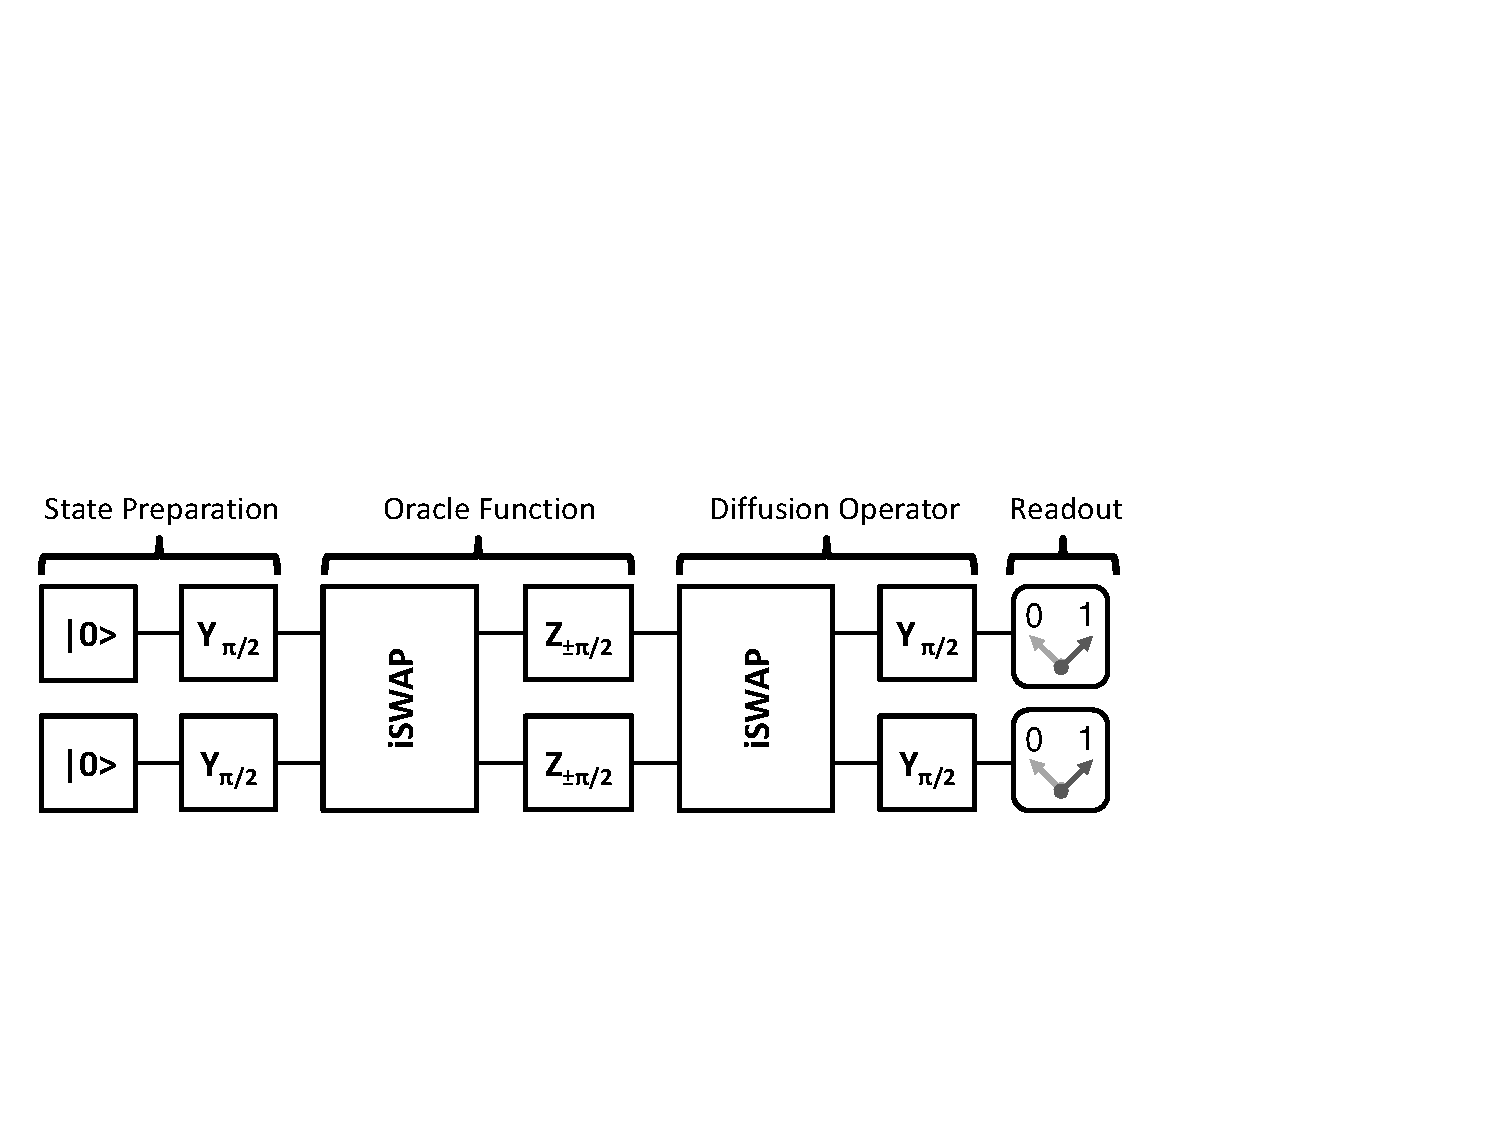
\includegraphics[width=\textwidth]{./material/papers/grover/grover_algorithm}
	\caption{Schematic of our implementation of the Grover search algorithm. The algorithm consists in generating a fully superposed input state, applying the Oracle function to it and analyzing the resulting state by applying the Diffusion transform and reading out the value of the qubit register afterwards.}
	\label{fig:GroverAlgorithmSchematic}
\end{figure}

The Grover algorithm has been implemented for two and three qubits using nuclear magnetic resonance (NMR) \citep{chuang_experimental_1998,vandersypen_implementation_2000} as well as for two qubits using trapped ions \citep{brickman_implementation_2005} and recently NV centers in diamond \citep{sar_decoherence-protected_2012}. In 2009, L. DiCarlo {\it et. al.} implemented it using a superconducting two-qubit processor \citep{dicarlo_demonstration_2009} achieving $>80 \%$ output state fidelity, albeit without using a sufficiently efficient readout scheme of the qubit register and therefore not being able to demonstrate quantum speed-up. The demonstration of quantum speed-up for the Grover search algorithm using a superconducting two-qubit processor with individual-qubit readouts is one of the main goals of this thesis work.

\smallskip

We implement the compiled version of the two-qubit Grover algorithm, which encodes the result of calling the Oracle function $\Or(x)$ with an input state $x$ directly in the phase of $x$, as described above. The gate sequence of the algorithm is shown in fig. \ref{fig:GroverAlgorithmSchematic} and consists of two $i\mathrm{SWAP}$ gates and six single-qubit gates applied to an initial state $\ket{00}$. Here, the first $i\mathrm{SWAP}$ gate (which includes a $Z_{\theta_I}^I\otimes Z_{\theta_{II}}^{II}$ gate sequence to compensate the acquired phases of the qubits) together with the two single-qubit $Z_{\pm \pi/2}$ rotations implements the Oracle function $\Or(x)$ as given by eq. (\ref{eq:two_qubit_oracle_operator}), where the signs of the rotation operations determines the state which is tagged by the Oracle ($--$, $-+$, $+-$ and $++$ for $\Or_{00}$, $\Or_{01}$, $\Or_{10}$ and $\Or_{11}$, respectively). This state can be either $\ket{00}$ (corresponding to a $Z^I_{-\pi/2}\cdot Z^{II}_{-\pi/2}$ rotation), $\ket{01}$ ($Z^I_{-\pi/2}\cdot Z^{II}_{\pi/2}$), $\ket{10}$ ($Z^I_{\pi/2}\cdot Z^{II}_{-\pi/2}$) or $\ket{11}$ ($Z^I_{\pi/2}\cdot Z^{II}_{\pi/2}$). After the encoding, the second $i\mathrm{SWAP}$ operation (which also includes Z compensation pulses) together with the following $X^I_{\pi/2}\cdot X^{II}_{\pi/2}$ single-qubit operations implements the diffusion operator as given by eq. (\ref{eq:two_qubit_diffusion_operator}). The final step of the algorithm consists in reading out the two-qubit register.

\subsection{Pulse Sequence}

\begin{figure}[ht!]
	\centering
		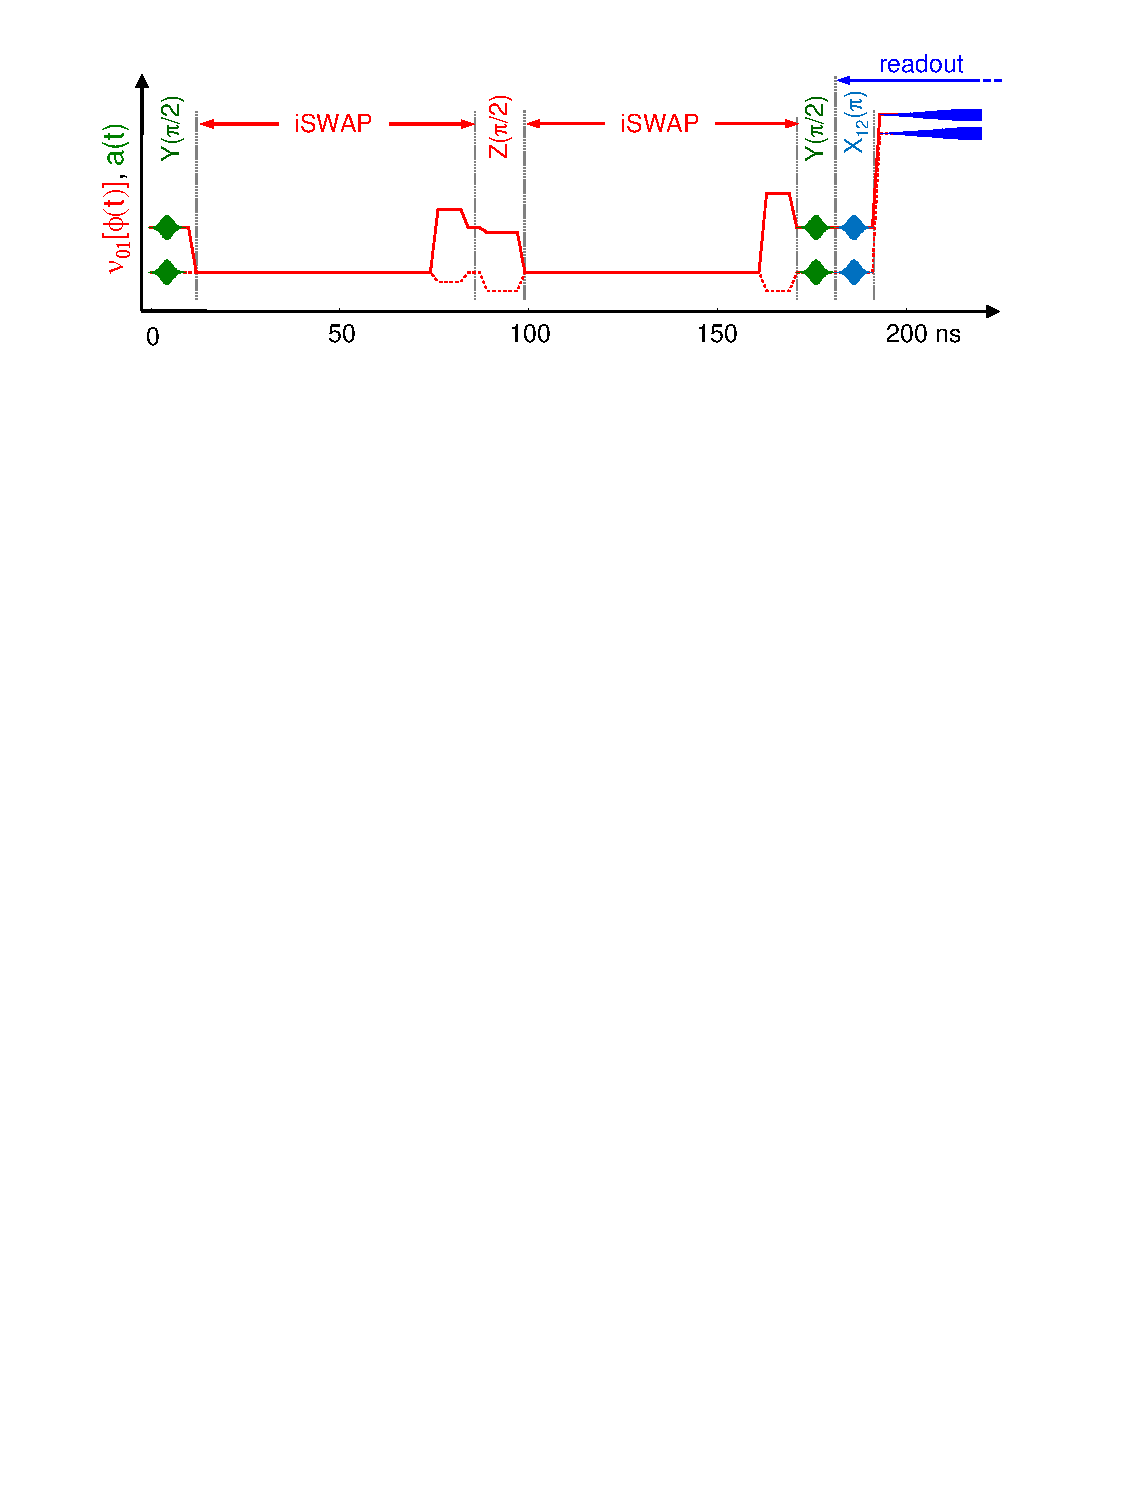
\includegraphics[width=0.95\textwidth]{./material/papers/grover/figures/grover_algorithm_pulse_sequence}
	\caption{Pulse sequence used to realize the two-qubit Grover quantum search algorithm. First, a $Y_{\pi/2}$ pulse is applied to each qubit to produce the fully superposed state $1/2(\ket{00}+\ket{01}+\ket{10}+\ket{11})$. Then, an $i\mathrm{SWAP}$ gate is applied, followed by a $Z_{\pm \pi /2}$ gate on each qubit, which combined correspond to the application of the Oracle function. The resulting state is then analyzed using another $i\mathrm{SWAP}$ gate and two $X_{\pi/2}$ gates to extract the state tagged by the Oracle. Optionally, a $Y^{12}_{\pi}$ pulse is applied to each qubit to increase the readout fidelity.}
	\label{fig:GroverPulseSequence}
\end{figure}

\begin{figure}[hp!]
	\centering
		\includegraphics[width=0.95\textwidth]{"./data/ct5/2011_04_21 - grover and tomo/good_data/grover algorithm - summary"}
	\caption{a) Schematic of the implemented algorithm, indicating the steps at which quantum state tomography has been performed. b) Experimental (filled circles) and theoretical (black outline) density matrices at different steps of the Grover search algorithm as indicated by the dotted lines, shown for four individual runs of the algorithm corresponding to different Oracle functions tagging the state ${\ket{00}}$, ${\ket{01}}$, ${\ket{10}}$ or ${\ket{11}}$. The trace fidelity (\ref{eq:quantum_trace_fidelity}) between experimental and theoretical density matrices is indicated above each matrix.}
	\label{fig:GroverAlgorithmExperimentalResults}
\end{figure}

We implement the gate sequence described above using microwave and fast flux pulses. To minimize gate errors, we perform a series of calibration measurements before to tune-up the individual single- and two-qubit gates needed for the algorithm, as explained in chapter \ref{chapter:processor_characterization}. In addition, we run individual parts of the algorithm successively and perform quantum state tomography to characterize the state of the quantum register after each step of the algorithm, optimizing the gate operations applied to the qubit in order to maximize the fidelity of the measured states in respect to the ideal ones. However, we optimize only the state preparation and Oracle operator itself on a per-state basis, whereas the diffusion operator $D$ is optimized only once for all possible Oracles, as required for benchmarking a real quantum algorithm. cases do not optimize the  Figure \ref{fig:GroverPulseSequence} shows an experimental pulse sequence for the Grover algorithm with an Oracle operator $\Or_{00}$. Shown are the frequencies of the two qubits during the run time of the algorithm and the microwave drive and readout pulses applied to them.

\section{Results}

We now present the experimental results obtained with our implementation of the Grover algorithm: Quantum state tomography is first used to determine the register density matrices during the algorithm, and single-run results are then presented and discussed.

\subsection{State Tomography of the Quantum Register}

Figure \ref{fig:GroverAlgorithmExperimentalResults}b shows the experimentally measured density matrices of the two-qubit register when running the Grover search algorithm for the four possible Oracle functions. For each of those four cases, quantum state tomography was performed after each step of the algorithm, as indicated in fig. \ref{fig:GroverAlgorithmExperimentalResults}a. The fidelity diminishes during the algorithm due to dephasing and relaxation. The state fidelities for the final output states of the algorithm are $68\%$ for the $\Or_{00}$, $64\%$ for the $\Or_{01}$, $61\%$ for the $\Or_{10}$ and $65\%$ for the $\Or_{11}$ Oracle functions.

\subsection{Single Run Results}

\begin{figure}[ht!]
	\centering
		\includegraphics[width=1.\textwidth]{"./data/ct5/2011_04_21 - grover and tomo/good_data/grover algorithm - single run probabilities"}
		\caption{Single-run success probabilities of our implementation of the Grover search algorithm, for the four possible Oracle functions. Red bars correspond to measured values, whereas blue ones are calculated using the measured density matrices after the final step of the algorithm and the measured two-qubit readout matrix as shown in fig. \ref{fig:GroverReadoutMatrix}. Dashed lines indicate the average success probabilities of classical query and query-and-guess algorithms, for comparison.}
	\label{fig:GroverSingleShotResults}
\end{figure}

The experimental state tomographies presented above show that we can implement the Grover search algorithm with average output state fidelity of 64 \% using our two-qubit processor. However, the analysis of the two-qubit register by quantum state tomography at the end of the algorithm does not prove that we can achieve real quantum speed-up with our processor. For this, it is necessary to directly read out the state of the qubit register at the end of the algorithm {\it without} performing any kind of error correction afterwards. By looking at this ``raw'' outcome data and generating statistics over many single runs of the processor, we quantify the success rate and the fidelity of the implemented algorithm. The results of such measurements, performed for the four possible Oracle functions, are shown in fig. \ref{fig:GroverSingleShotResults}. Besides the single-run probabilities for all four Oracle functions, the diagram shows for comparison the expected outcome probabilities calculated based on the quantum state tomographies discussed above and the readout matrix of the two-qubit processor shown in fig. \ref{fig:GroverReadoutMatrix}. As can be seen, the agreement between the measured and calculated probabilities is fairly good. Deviations between expected and measured outcome probabilities (such as for the $\ket{10}$ state when using the $C_{10}$ Oracle) might be explained by a drift of the experimental parameters between the measurement of the state tomographies and the single-run data. The dashed lines in the diagrams correspond to the success probabilities of classical single-evaluation query and query-and-guess algorithms, which are \mbox{25 \%} and \mbox{50 \%}, respectively, and which provide a benchmark against which we measure the quantum speed-up of our algorithm. Our implementation of the Grover search algorithm outperforms such classical algorithms for all Oracle functions, if only by 2-17 \% for the ``query-and-guess'' algorithm.


\section{Algorithm Fidelity}

\begin{table}[H]
\begin{centering}
\begin{tabular}{|c|c|c|c|c|c|c|}
\hline 
$ab$/$|uv\rangle$ & $\left|00\right\rangle $ & $\left|01\right\rangle $ & $\left|10\right\rangle $ & $\left|11\right\rangle $ & $\sum$ & $f_{ab}$\tabularnewline
\hline
\hline 
00 & \textcolor{red}{0.666} & 0.192 & 0.188 & 0.122 & 1.168 & 57.0 \%\tabularnewline
\hline 
01 & 0.127 & \textcolor{red}{0.554} & 0.071 & 0.122 & 0.874 & 63.4 \%\tabularnewline
\hline 
10 & 0.128 & 0.106 & \textcolor{red}{0.615} & 0.239 & 1.088 & 56.5 \%\tabularnewline
\hline 
11 & 0.079 & 0.148 & 0.126 & \textcolor{red}{0.517} & 0.870 & 59.4 \%\tabularnewline
\hline
\end{tabular}
\par\end{centering}

\caption{Conditional probabilities
$p_{ab/|uv\rangle}$ and user fidelities $f_{ab}$ for all
possible outcomes $ab$ for our implementation of Grover's algorithm.}
\label{tab:Probabilities-for-obtaining}
\end{table}

We define the average fidelity $f_i$ of the algorithm in a single run as the conditional probability of finding the correct state $\ket{i}$ given a certain Oracle function $\Or_i$. We also define {\it user fidelities}
%
\begin{equation}
f_{ab} = p(\ket{ab}|ab) = \frac{p(ab |\ket{ab})}{\sum\limits_{uv}p(uv|\ket{uv})},
\end{equation}
%
where $p(ab|\ket{ab})$ is the conditional probability of obtaining the search result $ab$ given the Oracle operator $\ket{ab}$. These user fidelities are complementary to the average fidelity and correspond to the conditional probabilities of having found the correct state given a certain measured state, averaged over all possible Oracle functions. For all four Oracles, both the single-run and user fidelities as shown in tab. \ref{tab:Probabilities-for-obtaining} are $> 50 \%$, hence demonstrating quantum speed-up in comparison with a classical query-and-guess algorithm.

\section{Comparison to a Classical Search Algorithm}

\begin{figure}[ht!]
	\centering
	\includegraphics[width=1\textwidth]{"./material/mathematica/comparision_grover_classical"}
	\caption{Comparison between our measured success probability of our implementation of the Grover algorithm and the calculated success probabilities of the query and query-and-guess classical algorithms as a function of the number $n$ of runs.}
	\label{fig:comparison_grover_classical}
\end{figure}

As discussed above, we compare our implementation of the Grover algorithm to the classical query and query-and-guess algorithms in order to quantify the quantum speed-up achieved. More precisely, we calculate the success probability of our algorithm to find the solution of the search problem after $n$ runs as
%
\begin{equation}
p_s(n) = \sum\limits_{i=1}^n (1-p_s^0)^{i-1}p_s^0,
\end{equation}
%
where $p_s^0$ is the single-run success probability of the algorithm. Figure \ref{fig:comparison_grover_classical} shows $p_s(n)$ for our implementation of the Grover algorithm as obtained for all four Oracle operators, together with the success probabilities of the query and query-and-guess classical algorithms. As can be seen, our implementation of the Grover algorithm beats the query algorithm for $n\le $3 evaluations of $\Or$ and the classical query-and-guess algorithm for $n\le 2$. However, unlike the classical algorithms, it never converges to 100 \% success probability due to always-present unitary and non-unitary errors in our system. 

\section{Error Analysis}

Three kind of errors arise in our implementation of the Grover algorithm:

\begin{enumerate}
	\item Deterministic, unitary gate errors.
	\item Stochastic errors introduced due to qubit decoherence.
	\item Readout errors (due to qubit relaxation during readout, insufficient readout sensitivity or retrapping of the readout resonator state).
\end{enumerate}

\subsection{Gate Errors \& Decoherence}

As far as gate errors and unitary errors are concerned, we quantify them by fitting an error model described below to the experimental data. In contrast to chapter \ref{chapter:processor_characterization}, where we used a full master-equation model to simulate the implemented $\sqrt{i\mathrm{SWAP}}$ gate, we use now an operator-based formalism to model the Grover algorithm with all relevant unitary and non-unitary errors in a simple and intuitive way. Hence, rather than performing a time-integration of an effective Hamiltonian, we start with an initial density matrix $\rho$ and apply a sequence of unitary gate operators $O_i$ to it in order to simulate the individual steps of the algorithm, including possible unitary gate errors. In addition, we approximate decoherence by inserting after each operation $O_i$ non-unitary relaxation and dephasing operators with rates $\Gamma_1$ or $\Gamma_\phi$ and duration $\Delta t_i$ equal to the duration of $O_i$ (note that dephasing is treated here in a phenomenological way, as discussed in section \ref{section:master_equation}). 

\smallskip

The non-unitary single-qubit operators describing amplitude-damping of the qubit state are \citep{nielsen_quantum_2000}
%
\begin{align}
 E_1^{\Gamma_1}(\Delta t) & = \left(\begin{array}{cc} 1 & 0 \\ 0 & \sqrt{1-\gamma_{\Gamma_1}(\Delta t)} \end{array}\right)   &  E_2^{\Gamma_1}(\Delta t)  & = \left( \begin{array}{cc} 0 & \sqrt{\gamma_{\Gamma_1}(\Delta t)} \\ 0 & 0 \end{array} \right), \label{eq:grover_energy_relaxation}
\end{align}
%
whereas phase-damping operators describing qubit dephasing are written as
%
\begin{align}
 E_1^{\Gamma_\phi}(\Delta t) & = \left(\begin{array}{cc} 1 & 0 \\ 0 & \sqrt{1-\gamma_{\Gamma_\phi}(\Delta t)} \end{array}\right)   &  E_2^{\Gamma_\phi}(\Delta t)  & = \left( \begin{array}{cc} 0 & 0 \\ 0 & \sqrt{\gamma_{\Gamma_\phi}(\Delta t)}  \end{array} \right). \label{eq:grover_phase_decoherence}
\end{align}
%
Both operators are applied to a quantum state $\rho$ according to
%
\begin{equation}
\rho \to \Er_{\Delta t}(\rho,E) = E_1(\Delta t)\rho E_1^\dagger(\Delta t)+E_2(\Delta t) \rho E_2^\dagger(\Delta t)
\end{equation}
%
and yield a trace-preserving, non-unitary evolution of the density matrix $\rho$. The decoherence fractions $\gamma$ used in the operators are given by
%
\begin{eqnarray}
\gamma_{\Gamma_{1}}(\Delta t) & =  & 1-\exp{\left(-\Delta t \Gamma_1\right)}, \label{eq:effective_relaxation_rate} \\
\gamma_{\Gamma_\phi}(\Delta t) & = & 1-\exp{\left(-\Delta t \Gamma_\phi/2\right)}, \label{eq:effective_dephasing_rate}
\end{eqnarray}
%
where $\Delta t$ is the time during which the state is exposed to the given decoherence process. Normally, decoherence processes occur continuously during the run time of the algorithm. However, in our simulation we apply the operators (\ref{eq:grover_phase_decoherence}) and (\ref{eq:grover_energy_relaxation}) to the quantum state at discrete times $\{t_1,\hdots,t_i,\hdots,t_n\}$, using effective decoherence rates $\gamma_{\Gamma_1}(\Delta t_i)$ and $\gamma_{\Gamma_\phi}(\Delta t_i)$ with $\Delta t_i = t_{i+1}-t_i$ to model the decoherence between times $t_{i}$ and $t_{i+1}$. In order for this approximation to be valid, the integration time $\Delta t_i$ needs to be small compared to the relaxation and dephasing times of the qubits, i.e. $\Delta t_i \ll 1/\Gamma_1,1/\Gamma_\phi$. We assure this by splitting up long unitary operators $O_i$ with duration $\Delta t_i$ into an equivalent sequence of $n$ operators $O_i^{1/n}$ with durations $\Delta_i t/n$, after each of which we apply the decoherence process using an adapted integration time $\Delta t_i/n$, as shown in fig. \ref{fig:error_model_trotterization}. If $n$ is chosen sufficiently large, the condition formulated above will always be fulfilled.

\begin{SCfigure}[1.0][ht!]
	\centering
	\includegraphics[width=0.5\textwidth]{"./material/papers/grover/error_model_trotterization"}
	\caption{Finite difference model of a unitary gate sequence $O$ with a duration $\Delta t$ that is subjected to a decoherence process with rate $\gamma(\Delta t)$: The evolution operator $O$ is split into a sequence of $n$ operators $O^{1/n}$, each of which is subjected to a decoherence process with an effective rate $\gamma(\Delta t/n)$.}
	\label{fig:error_model_trotterization}
\end{SCfigure}

\smallskip

Using these definitions, we formulate a full error model taking into account the following error sources:

\begin{itemize}
 \item {\bf Energy relaxation and dephasing}: Energy relaxation and dephasing of the qubits is modeled by applying the operators given by eqs. (\ref{eq:grover_energy_relaxation}) and (\ref{eq:grover_phase_decoherence}) with rates (\ref{eq:effective_relaxation_rate}) and (\ref{eq:effective_dephasing_rate}) to the quantum state after each unitary operator during the algorithm. Operators with an experimental duration larger than $\Delta t_\mathrm{max}=5\;\mathrm{ns}$ are split up into a sequence of sub-operators with durations $\Delta t \le \Delta t_\mathrm{max}$, where we apply the decoherence process after each of these sub-operators.
 \item {\bf Single-qubit gate errors}: Rotation angle and axis errors of the single-qubit $X_\alpha$ and $Y_\alpha$ gates are modeled by replacing them with operators of the form $X_\alpha\to \phi_{\alpha'} = \cos{\phi}X_{\alpha'}+\sin{\phi}Y_{\alpha'}$ and $Y_\alpha \to \varphi_{\alpha'} = \sin{\varphi}X_{\alpha'}+\cos{\varphi}Y_{\alpha'}$. For $Z$-type single-qubit operators, we have only rotation angle errors by replacing $Z_\beta \to Z_{\beta'}$ 
 \item {\bf Two-qubit gate errors:} Errors in the $i\mathrm{SWAP}$ operator are modeled using the representation of the iSWAP gate given by eq. (\ref{eq:swap_with_detuning}), replacing $t$ and $\Delta$ with $\epsilon = t g_{e}$ and $\delta = \Delta / g$. In addition, we model the errors in the $Z$ compensation pulses by including single-qubit rotations of the form $Z_{\theta_I}^I\otimes Z_{\theta_{II}}^{II}$.
\end{itemize}

\begin{figure}[hp!]
	\centering
		\includegraphics[width=\textwidth]{"./data/ct5/2011_04_21 - grover and tomo/good_data/grover - simulated density matrices with errors - with schematic"}
	\caption{a) Schematic of the unitary error model given by eq. (\ref{eq:grover_error_model}), which we use to analyze our experimental implementation of the Grover search algorithm. Dotted lines indicate the times at which the quantum state has been measured by state tomography. The execution time of the experimental sequence implementing each operator is indicated above it. b) Experimentally measured density matrices at different times during the algorithm (black outlines) together with matrices corresponding to the best fit of the error model (filled circles) to the data, plotted for four individual runs of the algorithm corresponding to different Oracle operators. The state fidelity between the measured and simulated density matrices is indicated above each panel.}
	\label{fig:GroverErrorModel}
\end{figure}

The full algorithm with unitary and non-unitary errors and taking into account all gate times can be written as
%
\begin{eqnarray}
O_\mathrm{Grover}(\rho) & = & O_7(O_6(O_5(O_4(O_3(O_2(O_1(\rho))))))) \label{eq:grover_error_model} \\
O_1(\rho) & = & \De^{\times 2}_{5\;\mathrm{ns}}\left(\left[\varphi_{\alpha_I}^I\otimes \varphi_{\alpha_{II}}^{II}\right]^{1/2},\rho\right) \notag \\
O_2(\rho) & = & \De^{\times 16}_{3.875\;\mathrm{ns}}\left(i\mathrm{SWAP}(\epsilon_1,\delta_1)^{1/16},\rho\right) \notag \\
O_3(\rho) & = & \De_{5\;\mathrm{ns}}\left(Z_{\theta_I}^I\otimes Z_{\theta_{II}}^{II},\rho\right) \notag \\
O_4(\rho) & = & \De_{5\;\mathrm{ns}}\left(Z_{\beta_I}\otimes Z_{\beta_{II}},\rho\right) \notag \\ 
O_5(\rho) & = & \De^{\times 16}_{3.875\;\mathrm{ns}}\left(i\mathrm{SWAP}(\epsilon_2,\delta_2)^{1/16},\rho\right) \notag \\ 
O_6(\rho) & = & \De_{5\;\mathrm{ns}}\left(Z_{\lambda_I}^I\otimes Z_{\lambda_{II}}^{II},\rho\right) \notag \\
O_7(\rho) & = & \De^{\times 2}_{5\;\mathrm{ns}}\left(\left[\phi_{\gamma_I}^I\otimes \phi_{\gamma_{II}}^{II}\right]^{1/2},\rho\right), \notag
\end{eqnarray}
%
where $\De_{\Delta t}(M,\rho)=\Er_{\Delta t}(\Er_{\Delta t}(\Er_{\Delta t}(\Er_{\Delta t}(M\rho M^\dagger,E^{\Gamma_1^I}\otimes \mathrm{I}),E^{\Gamma_\phi^I}\otimes \mathrm{I}),\mathrm{I}\otimes E^{\Gamma_1^{II}}),\mathrm{I}\otimes E^{\Gamma_\phi^{II}})$ and $\De_{\Delta t}^{\times n}(M,\rho)$ is the $n$-fold recursive application of $\De_{\Delta t}(M,\cdot)$ to $\rho$. Figure \ref{fig:GroverErrorModel}a shows a schematic of this sequence, indicating above each operator its duration. Numerical optimization is used to fit this error model to the experimentally obtained density matrices measured after each step of the algorithm, as obtained in four individual runs using different Oracle operators tagging the states $\ket{00}$, $\ket{01}$, $\ket{10}$ and $\ket{11}$. We fit the parameters of the operators $O_i$ that model each individual step $i$ of the algorithm by maximizing the fidelity between the experimentally obtained output density matrix $\rho_{i}^\mathrm{exp}$ of the step and the modeled one $\rho_i^\mathrm{mod}$, which is calculated based on the experimental input density matrix $\rho_{i-1}^\mathrm{exp}$ as $\rho_{i}^\mathrm{mod} = O_i(\rho_{i-1}^\mathrm{exp})$. For the first step, we set the input state to $\rho^\mathrm{exp}_0=\ket{00}\bra{00}$. The parameters of the operators $O_i$ are not allowed to vary between the four different runs, except for $\beta_{I,II}$, which were adjusted independently for each Oracle operator. This yields in total 24 parameters that are fitted to a data set containing 20 density matrices, each corresponding to 15 measured real values. The density matrices corresponding to the best fit together with the experimentally measured matrices are shown in fig. \ref{fig:GroverErrorModel}b. The obtained error parameters are summarized in tab. \ref{tab:grover_error_parameters}. As before, the qubit relaxation and dephasing rates of $\Gamma_1^I = (436\;\mathrm{ns})^{-1}$, $\Gamma_1^{II}=(520\;\mathrm{ns})^{-1}$, $\Gamma_\phi^I=\Gamma_\phi^{II}=(600\;\mathrm{ns})^{-1}$ were determined independently and are not part of the fit.

\begin{table}[ht!]
\begin{tabular}{r|rrrrrrrr}
value & $\alpha_I (^\circ)$ & $\alpha_{II} (^\circ)$ & $\varphi_I (^\circ)$ & $\varphi_{II} (^\circ)$ & $\epsilon_I (^\circ)$ & $\epsilon_{II} (^\circ)$ & $\theta_{I} (^\circ)$ & $\theta_{II} (^\circ)$\\ \hline
absolute  & 93.4 & 88.2 & 101.5  &  96.8 & 88.7  & 96.6  & -19.8 & -20.8 \\
deviation  & (3.4) & (-1.8) & (11.5) & (6.8)  & (-1.3) & (6.6) & (-19.8) & (-20.8) \bigskip \\ 
& $\delta_I\;(\mathrm{MHz})$ & $\delta_{II}\;(\mathrm{MHz})$ & $\gamma_I (^\circ)$ & $\gamma_{II} (^\circ)$ & $\phi_I (^\circ)$ & $\phi_{II} (^\circ)$ & $\lambda_{I} (^\circ)$ & $\lambda_{II} (^\circ)$ \\ \hline
absolute & -0.128 & 0.181 & 87.2 & 91.2 & -1.0 & -5.0 & 8.7 & 4.6 \\
deviation & (-0.128) & (0.181) & (-2.8) & (1.2) & (-1.0) & (-5.0)  & (8.7) & (4.6)
\end{tabular} \bigskip \\ 
\begin{tabular}{p{1cm}r|rrrr}
run & & $\Or_{00}$ & $\Or_{01}$ & $\Or_{10}$ & $\Or_{11}$ \\ \hline
\multicolumn{1}{r}{$\beta_I (^\circ)$} & & -92.4 (-2.4) & 90.2 (0.2) & -92.9 (-2.9) & 87.3 (-2.7)   \\
\multicolumn{1}{r}{$\beta_{II} (^\circ)$} & & -98.1 (-8.1) & -94.0 (-4.0) & 81.4 (-8.6) & 77.5 (-12.5)  
\end{tabular}
\caption{Shown are the absolute values and deviations (in parenthesis) of the parameters of the error model given by eq. (\ref{eq:grover_error_model}) for the measured density matrices.}
\label{tab:grover_error_parameters}
\end{table}

%#Optimized parameters 1: [-86.640820735407374, 88.195343671067462, -78.515727923642544, 96.840572880579657]
%#Optimized parameters 2: [88.720303371532054, -7.3431185025239643, 160.26477098328292, 159.19317605817503]
%#Optimized parameters 3-1: [-92.39344544657115, -98.066825154157868]
%#Optimized parameters 3-2: [90.168548505116462, -94.260980331193991]
%#Optimized parameters 3-3: [-92.871592140562313, 81.363510506368826]
%#Optimized parameters 3-4: [87.306170896838864, 77.526144982079813]
%#Optimized parameters 4: [-83.405879395949796, 10.389588676233945, 8.6895247351201874, 4.6363430474926872]
%#Optimized parameters 5: [-92.828226992303087, 91.220254404928369, -179.0202560696969, -4.9601230810921493]

Our error model is able to capture most of the observed experimental errors and can reproduce to a large extent the observed density matrices. The state fidelities according to eq. \ref{eq:quantum_state_fidelity} between the measured density matrices and those of the fitted error model are all $\ge 97\%$. The rotation angle and axis errors of the $X/Y$ pulses vary between $\pm3^\circ$ and $\pm 12^\circ$, respectively, which is comparable with the single-qubit gate errors estimated in chapter \ref{chapter:processor_characterization}. The errors in the $Z$ rotations are considerably larger and vary between $\pm 20^\circ$, which can be explained by the reduced accuracy with which we calibrate these gates and by a drift of our measurement equipment during the experiment, as described in section \ref{section:bell_inequality}.

\smallskip

Given the large number of fitting parameters and the phenomenological treatment of dephasing, these results can suffer from large uncertainties and only show the order of magnitude of different errors and their impact on the register density matrices along the algorithm.

\subsubsection{Fidelity of the Oracle and Diffusion Operators}

It is interesting to analyze the individual output state fidelities of the Oracle and diffusion operators. For this, we compare the action of the ideal operators $D$ and $R$ given by eqs. (\ref{eq:two_qubit_diffusion_operator}) and (\ref{eq:two_qubit_oracle_operator}) on a given input state with that of the experimentally implemented ones. We do this by applying the ideal operators $D$ and $R$ to their experimentally measured two-qubit input density matrices $\rho^\mathrm{exp}_{\mathrm{in},D,R}$ and calculating the fidelity of the resulting matrices with the experimentally obtained output matrices $\rho_{\mathrm{out},D,R}^\mathrm{exp}$:
%
\begin{eqnarray}
F(D) & = & F(D\rho_{\mathrm{in},D}^\mathrm{exp}D^{\dagger},\rho_{\mathrm{out},D}^\mathrm{exp}), \label{eq:grover_diffusion_fidelity} \\
F(R) & = & F(R\rho_{\mathrm{in},R}^\mathrm{exp}R^{\dagger},\rho_{\mathrm{out},R}^\mathrm{exp}), \label{eq:grover_oracle_fidelity}
\end{eqnarray}
%
where we make use of the state fidelity $F$ given by eq. \ref{eq:quantum_state_fidelity}. By this method, we obtain the following experimental fidelities for the Oracle and diffusion operations:

\begin{table}[ht!]
\centering
\begin{tabular}{r|rrrr|l}
Operator / State & $\ket{00}$ & $\ket{01}$ & $\ket{10}$ & $\ket{11}$ & Average \\ \hline 
$D$ & 92.3 & 93.4 & 94.3 & 91.7 & 92.9 \\
$R$ & 94.5 & 93.6 & 88.5 & 87.7 & 91.1
\end{tabular}
\caption{Measured fidelities (in \%) of the quantum Oracle and diffusion operators used in the Grover search algorithm according to eqs. (\ref{eq:grover_diffusion_fidelity}) and (\ref{eq:grover_oracle_fidelity}).}
\end{table}

As can be seen, we are able to implement both the diffusion operator and the quantum Oracle with an average fidelity $>90\%$.

\subsection{Readout Errors}

\begin{SCfigure}[1.0][ht!]
	\centering
\includegraphics[width=0.5\textwidth]{"./data/ct5/2011_04_21 - grover and tomo/good_data/readout only"}
	\caption{The measured readout matrix for the Grover experiment. Shown are the conditional probabilities $p_m(x|y)$ of obtaining a readout value $x$ after having prepared a qubit state $\ket{y}$, where $x,y\in\{00,01,10,11\}$. The readout fidelities for the different qubit states range between 75 - 88 \%, the inter-qubit readout crosstalk ranges between 3-5 \%.}
	\label{fig:GroverReadoutMatrix}
\end{SCfigure}

Another direct source of errors affecting the single-run fidelities of the algorithm are readout errors. As explained in chapter \ref{chapter:measurement} qubit relaxation during the readout process reduces the visibility of individual qubit states and introduces errors when reading out the qubit register in the final step of the algorithm. We can easily quantify those readout errors by using the readout matrix that was introduced in chapter \ref{chapter:processor_characterization}. When running the Grover algorithm, we use the $\ket{1}\to\ket{2}$ shelving method described in chapter \ref{chapter:measurement} to increase the readout contrast and thereby the algorithm fidelity. This technique reduces single-qubit readout errors but increases inter-qubit readout crosstalk. The measured readout matrix for the Grover experiment is shown in fig. \ref{fig:GroverReadoutMatrix}. As can be seen, the single-qubit readout fidelities range between 87 - 96 \% and the combined two-qubit readout fidelities between 75 - 88 \%. Depending on the qubit state we also observe between 3-5 \% inter-qubit readout crosstalk.

\section{Conclusions}

We have shown that we can implement the Grover search algorithm with our quantum processor and achieve a single-run fidelity that is sufficient to demonstrate simple probabilistic quantum speed-up, as compared to a classical, reversible search algorithm. The error model formulated in this chapter is able to account for most of the observed imperfections and can explain the data we observed. Unfortunately, the coherence times of our qubits do not permit the realization of more complex algorithms with our processor, but nevertheless it provides a proof-of-principle of our approach to build a superconducting quantum computer with individual-qubit single shot readout.
